\documentclass[border=10pt]{standalone}
\usepackage{pgfplots}
\pgfplotsset{compat=1.18, trig format plots=rad}
\begin{document}
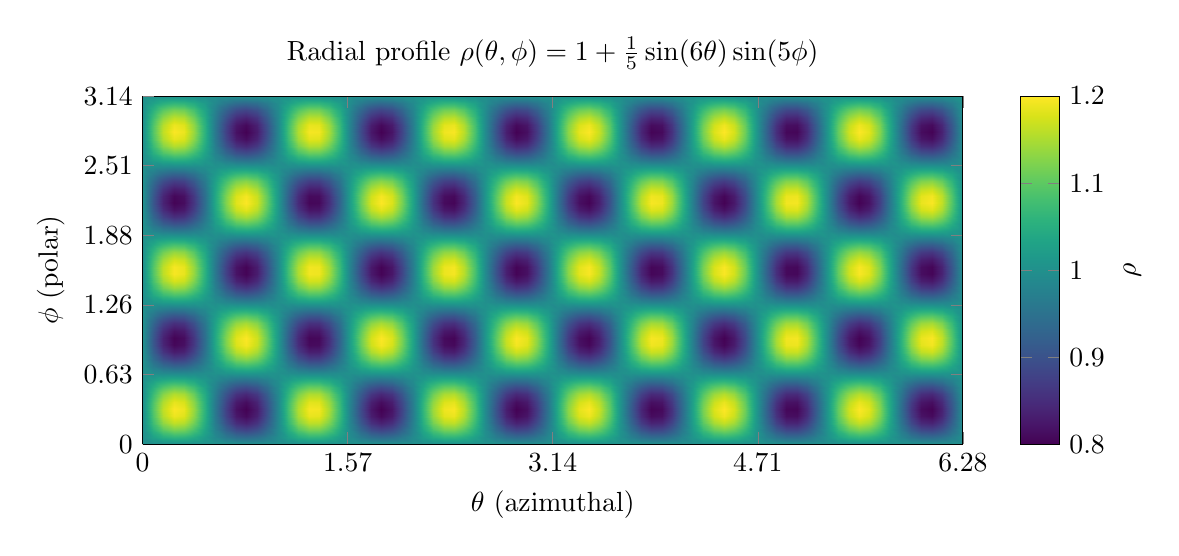
\begin{tikzpicture}
\begin{axis}[
    width=12cm, height=6cm,
    view={0}{90},
    xlabel={$\theta$ (azimuthal)},
    ylabel={$\phi$ (polar)},
    xtick={0, pi/2, pi, 3*pi/2, 2*pi},
    ytick={0, pi/5, 2*pi/5, 3*pi/5, 4*pi/5, pi},
    colormap/viridis,
    colorbar,
    colorbar style={
        ylabel={$\rho$},
    },
    enlargelimits=false,
    title={Radial profile $\rho(\theta,\phi)=1+\frac{1}{5}\sin(6\theta)\sin(5\phi)$},
]
\addplot3[
    surf,
    shader=interp,
    samples=80,
    samples y=50,
    domain=0:2*pi,
    y domain=0:pi,
    point meta={1+0.2*sin(6*x)*sin(5*y)},
] {1+0.2*sin(6*x)*sin(5*y)};
\end{axis}
\end{tikzpicture}
\end{document}